\documentclass{scrartcl}
\usepackage[a4paper,left=1in,right=1in,top=1.2in,bottom=1in]{geometry}
\usepackage{siunitx}
\usepackage{graphicx}
\setkomafont{disposition}{\normalfont\bfseries}

%title
\title{Exercise 02:\\Single-compartment model}
\subtitle{Theoretical Neuroscience I}
\author{Johannes G\"atjen}

%use these for structure/overview
\newcommand\Question{%
  \textbf{Question:}%
}
\newcommand\Answer{%
  \textbf{Answer:}%
}

\begin{document}
\maketitle
\Question\\
Compute and plot the dependent variables of a neuron with the single-compartment model for a constant input current, an oscillating input current with low frequency (10\si{Hz}), an oscillating input current with medium frequency (100\si{Hz}) and a high frequency random input current. Use the following values for the independent variables: $r_m = 0.9\si{\mega\ohm\square\milli\meter}$, $c_m = 12\si{\nano\farad\per\square\milli\meter}$, $V_0 = 0\si{mV}$ and $i_0 = 25 \si{\nano\ampere\per\square\milli\meter}$.
\\\\
\Answer\\
\begin{figure}[h]
\centering
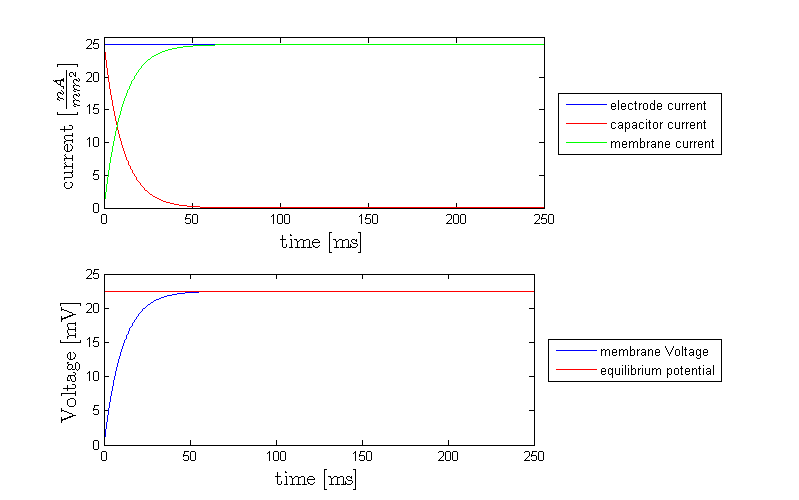
\includegraphics[trim = {1.3cm 0 2cm 0.9cm}, width=\textwidth, clip]{../pics/constant}
\caption{\small{Constant input current: $i_e(t) = i_0$ Top: The electrode current($i_e$, blue), the capacitor current($i_c$, red) and the membrane current ($i_r$, green) over time. Bottom: The membrane voltage ($V_m$, blue) and the equilibrium potential ($V_\infty$, red) over time.}}
\label{constant}
\end{figure}


\begin{figure}
\centering
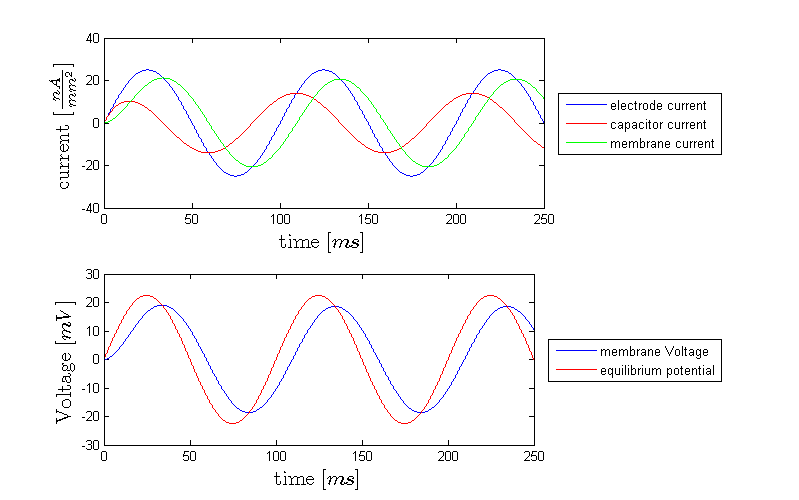
\includegraphics[trim = {1.3cm 0 2cm 0.9cm}, width=\textwidth, clip]{../pics/low}
\caption{\small{Low frequency input current: $i_e(t) = i_0 \cdot \sin{2\pi f t}$ , $f = 10\si{\hertz}$} Same variables shown as in Figure \ref{constant}.}
\end{figure}

\begin{figure}
\centering
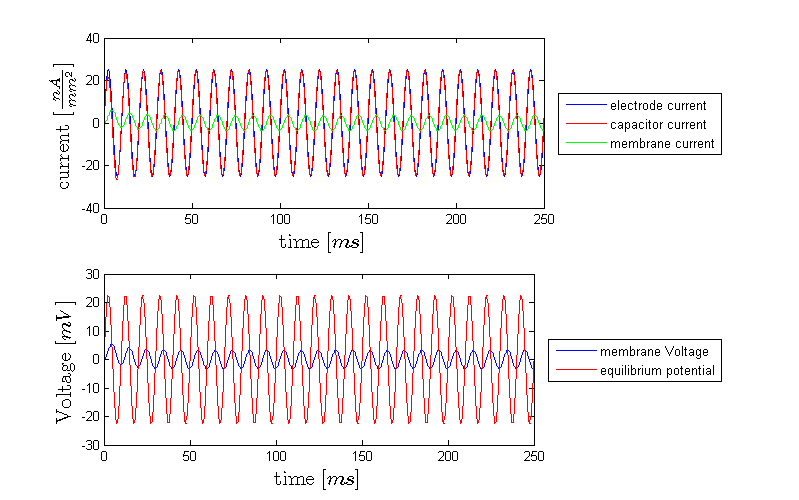
\includegraphics[trim = {1.3cm 0 2cm 0.9cm}, width=\textwidth, clip]{../pics/medium}
\caption{\small{Medium frequency input current: $i_e(t) = i_0 \cdot \sin{2\pi f t}$ , $f = 100\si{\hertz}$} Same variables shown as in Figure \ref{constant}.}
\end{figure}

\begin{figure}
\centering
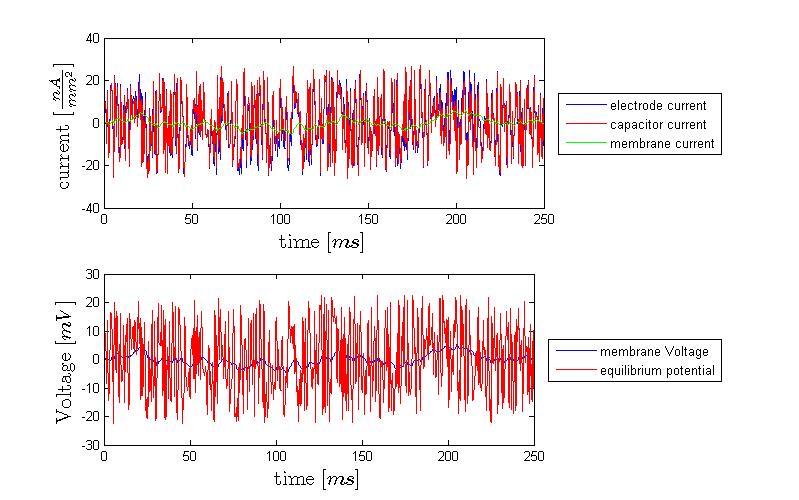
\includegraphics[trim = {1.3cm 0 2cm 0.9cm}, width=\textwidth, clip]{../pics/random}
\caption{\small{High frequency random input current. Same variables shown as in Figure \ref{constant}.}}
\end{figure}


\end{document}